\section{Analysis} 

\begin{frame}{Variable Selection}
\vspace{0.5 cm}
        \textbf{Removed before selection}
        \begin{itemize}
            \item Categorical covariates
            \item Covariates linked to employment aspects (such as \texttt{empl\_rate}, \texttt{part\_rate}, etc.)
        \end{itemize}
        \textbf{First selection} \\
        
        \begin{itemize}
            \item Remove redundant predictors that are very highly correlated:

            \[
                |\rho_{jk}| \ge 0.90
            \]
        \end{itemize}
\end{frame}


\begin{frame}{Variable Selection}
\textbf{Preprocessing}
    \begin{itemize}
        \item Start from the reduced set of covariates $X \in \mathbb{R}^{n \times p}$, after correlation-based filtering
        \item Standardized predictors and link function:
        \[
            X^{\ast}_{ij} = \frac{X_{ij} - \bar{X}_j}{s_{X_j}} \, , 
            \qquad
            y^{\ast}_i = \text{logit}(y_i) = \log\!\left( \frac{y_i}{1 - y_i} \right)
        \]

        \item Define an offset $o_i=\text{logit}(\texttt{mal\_empl\_rate}_i)$ to add to the regression model, so that it explains female employment relative to male employment.
    \end{itemize}
\end{frame}


\begin{frame}{Variable Selection - Frequentist Lasso}
    \begin{columns}[T]
        \column{0.7\textwidth}
            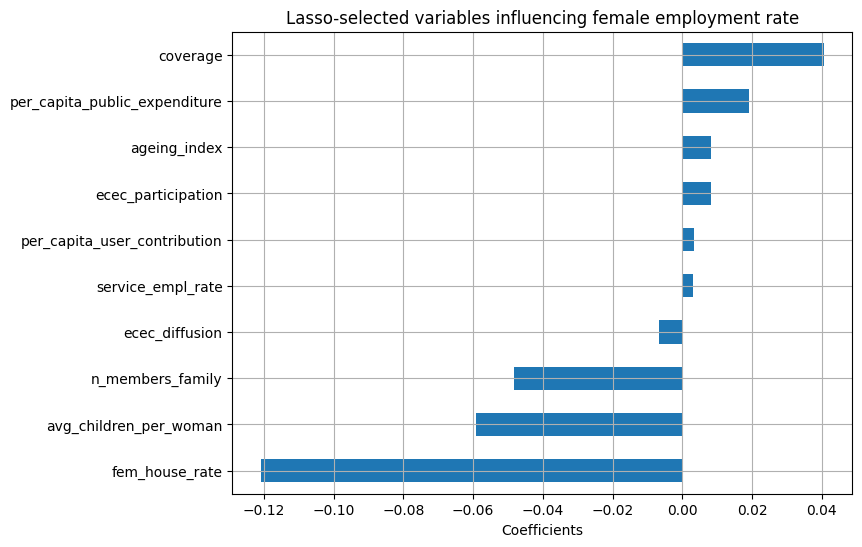
\includegraphics[scale=0.45]{pictures/coefs_freq_lasso.png}
    
        \column{0.3\textwidth}
            \textbf{Model} :\vspace{2mm} $y_i^{\ast} = \alpha + {x_i^{\ast}}^T\,\boldsymbol{\beta}  + o_i $\\ \vspace{2mm}
            for $ i = 1, \ldots, n$
                
             $\newline$
             \vspace{2mm}
            10 selected variables (5 ECEC covariates)\\
             $\newline$
             
            \vspace{2mm}
            $R^2: 0.553 \, ± \, 0.169$\\
             $\newline$        
    \end{columns}

\end{frame}


\newcommand{\iid}{\stackrel{\tiny{iid}}{\sim}}
\newcommand{\ind}{\stackrel{\tiny{ind}}{\sim}}

\begin{frame}{Variable Selection - Bayesian Lasso}
\footnotesize
    \begin{itemize}
        \item Bayesian Lasso regression model \cite{bayesianLasso}:
            \begin{align*}
                y^{\ast}_i \mid \boldsymbol{\beta}, \sigma 
                    &\stackrel{\text{ind}}{\sim}\mathcal{N}\big(\alpha +  x_i^{\ast \top} \boldsymbol{\beta} + o_i,\, \sigma^2\big) \, ,
                    \quad i = 1,\dots,n, \\
                \beta_j \mid \lambda, \sigma 
                    &\stackrel{\text{iid}}{\sim}\mathrm{Laplace}\big(0,\, \sigma / \lambda\big) \, ,
                    \quad j = 1,\dots,p \\
                \lambda^2 &\sim \mathrm{Gamma}(2, 1) \\
                \sigma &\sim \mathrm{HalfNormal}(1) \\
                \alpha &\sim \mathcal{N}\big(0, \, 10^2)
            \end{align*}
        \item Posterior sampling via MCMC (PyMC) for all $\beta_j$
        \item Variable selection rule:
        \begin{itemize}
            \item Compute 90\% credible intervals for each $\beta_j$
            \item Keep covariates whose 90\% credible interval does \underline{not} contain $0$
        \end{itemize}
    \end{itemize}        
\end{frame}

\begin{frame}{Variable Selection - Bayesian Lasso Results}
    \begin{center}
         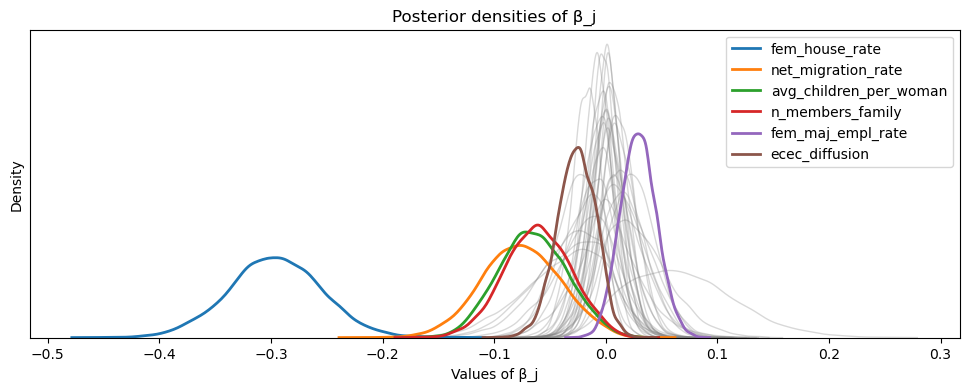
\includegraphics[scale=0.47]{pictures/beta_posterior.png}

         
         \footnotesize Selected Variables: \scriptsize \texttt{fem\_house\_rate, net\_migration\_rate, \\ avg\_children\_per\_woman, n\_members\_family, fem\_maj\_empl\_rate, ecec\_diffusion}.
    \end{center}
\end{frame}


\begin{frame}{Variable Selection - Comparison}

    \begin{table}[h!]
    \centering
    \footnotesize
        \begin{tabular}{lcc}
            \hline
            \textbf{Variable selected} & \textbf{Frequentist Lasso} & \textbf{Bayesian Lasso} \\
            \hline
            fem\_house\_rate                  & X & X \\
            net\_migration\_rate             &  & X \\
            avg\_children\_per\_woman        & X & X \\
            n\_members\_family               & X & X \\
            fem\_maj\_empl\_rate             &  & X \\
            \textbf{ecec\_diffusion}                  & X & X \\
            \textbf{per\_capita\_public\_expenditure} & X &  \\
            \textbf{ecec\_participation}              & X &  \\
            \textbf{coverage}                         & X &  \\
            \textbf{per\_capita\_user\_contribution}  & X &  \\
            ageing\_index                    & X &  \\
            service\_empl\_rate              & X &  \\
            \hline
        \end{tabular}
    \end{table}

\end{frame}